


%%%%%%%%%%%%%%%%%%%%%%%%%%%%%%%%%%%%%%%%%%%%%%%%%%%%%%%%%%%%%%%%%%%%%%%%%%%%%
%%%%%%%%%%%%%%%%%%%%%%%%%%%%%%%%%%%%%%%%%%%%%%%%%%%%%%%%%%%%%%%%%%%%%%%%%%%%%
%%%%%%%%%%%%%%%%%%%%%%%%%%%%%%%%%%%%%%%%%%%%%%%%%%%%%%%%%%%%%%%%%%%%%%%%%%%%%



\section{Selfish objects and classes}
\label{S:self}

In the previous section we have avoided one important tenet of OO: the
ability of methods to send messages to `self'.  One \emph{could}
simulate such selfish messages by implementing methods as regular
mutually recursive functions. Sending a message to `self' will then
clearly look differently than sending a message to another object. A
more important problem with that naive solution is the closed nature
of the method recursion. Overriding methods in subclasses will not
affect this recursion, drastically limiting subtype polymorphism.

So we need to bind `self' explicitly. Consequently, object templates
need to be in the style of `open recursion': they take self and
construct (some part of) self. This makes object templates amenable to
inheritance including subtype polymorphism. The following batch of
examples is mostly adopted from the OCaml tutorial. The source code
distribution for this paper contains many additional
examples~\cite{OOHaskell}.



%%%%%%%%%%%%%%%%%%%%%%%%%%%%%%%%%%%%%%%%%%%%%%%%%%%%%%%%%%%%%%%%%%%%%%%%%%%%%
%%%%%%%%%%%%%%%%%%%%%%%%%%%%%%%%%%%%%%%%%%%%%%%%%%%%%%%%%%%%%%%%%%%%%%%%%%%%%
%%%%%%%%%%%%%%%%%%%%%%%%%%%%%%%%%%%%%%%%%%%%%%%%%%%%%%%%%%%%%%%%%%%%%%%%%%%%%



\subsection{Object creation boils down to fix-point computation}

Quoting from~\cite[\S\,3.2]{OCaml}:

\begin{quote}\itshape
``A method or an initialiser can send messages to self (that is, the
current object). For that, self must be explicitly bound, here to the
variable @s@ (@s@ could be any identifier, even though we will often
choose the name @self@.)

...

\noindent
Dynamically, the variable s is bound at the invocation of a method. In
particular, when the class @printable_point@ is inherited, the
variable @s@ will be correctly bound to the object of the subclass.''
\end{quote}

\antiskip

\begin{code}
 class printable_point x_init =
   object (s)
     val mutable x = x_init
     method getX = x
     method move d = x <- x + d
     method print = print_int s#getX
   end;;
\end{code}

\noindent
Again, this OCaml code is transcribed to Haskell very directly. A
noteworthy and appreciated deviation is that @s@ ends up as just an
\emph{ordinary} argument of the monadic function for constructing
printable point objects:

\begin{code}
 printable_point x_init s =
   do
      x <- newIORef x_init
      returnIO
        $  mutableX .=. x
       .*. getX     .=. readIORef x
       .*. move     .=. (\d -> modifyIORef x ((+) d))
       .*. print    .=. ((s # getX ) >>= Prelude.print)
       .*. emptyRecord
\end{code}

\noindent
Object creation and invocation looks as follows in OCaml:

\begin{code}
 let p = new printable_point 7;;
 val p : printable_point = <obj>
\end{code}
 
\begin{code}
 p#move 2;;
 - : unit = ()
\end{code}

\begin{code}
 p#print;;
 9- : unit = ()
\end{code}

\noindent
We note that @s@ does not show up in the OCaml line that constructs a
point @p@ with the @new@ construct, but it is clear that the recursive
knot is tied right there. The Haskell code makes this really explicit.
We do not use any special @new@ construct. We simply use the (monadic)
fix-point operation as is:

\begin{code}
 mySelfishOOP =
   do
      p <- mfix (printable_point 7)
      p # move $ 2
      p # print
\end{code}

\begin{code}
 ghci> mySelfishOOP
 9
\end{code}



%%%%%%%%%%%%%%%%%%%%%%%%%%%%%%%%%%%%%%%%%%%%%%%%%%%%%%%%%%%%%%%%%%%%%%%%%%%%%
%%%%%%%%%%%%%%%%%%%%%%%%%%%%%%%%%%%%%%%%%%%%%%%%%%%%%%%%%%%%%%%%%%%%%%%%%%%%%
%%%%%%%%%%%%%%%%%%%%%%%%%%%%%%%%%%%%%%%%%%%%%%%%%%%%%%%%%%%%%%%%%%%%%%%%%%%%%



\subsection{Some MAJOR byproducts of using Haskell}

We would like to highlight some pieces of expressiveness and some
issues of convenience that are implied by our use of Haskell as the
base language for OO programming. The combined list that follows is
not covered by any mainstream OO language. This strongly suggests that
(OO)Haskell lends itself as a language-design environment.



\paragraph*{Type inference}

This claim stands: we haven't seen \emph{any} type annotations for
classes or methods or attributes so far. We will need annotations for
some purposes later. The reader may be interested how the inferred
types look like; we show the inferred type for a class inherited from
|point_class| below.



\paragraph*{First-class classes}

Using higher-order functional programming, we can programme functions
that take classes as arguments, compute them, instantiate them, use
them. The first-class status of classes is easily illustrated as
follows:

\begin{code}
 myFirstClassOOP point_class =
   do
      p <- mfix (point_class 7)
      p # move $ 35
      p # print
\end{code}
%%% $
\begin{code}
 > myFirstClassOOP printable_point
 42
\end{code}

\noindent
That is, we have parameterised @myFirstClassOOP@ in a class.



\paragraph*{Reusable methods}

Using some bits of parameterisation and higher-order functional
programming, we can programme methods outside of any hosting
class. Such methods can be reused across classes without any
inheritance relationship.  For instance, let's identify a method
@print_getX@ that can be shared by all objects that have at least the
method @getX@ of type @Show@~@a@~@=>@~@IO@~@a@~---~regardless of any
inheritance relationships:

\begin{code}
 print_getX self = ((self # getX ) >>= Prelude.print)
\end{code}

\noindent
We can update the corresponding line of @printable_point@ as follows:

\begin{code}
 -- before
 ... .*. print    .=. ((s # getX ) >>= Prelude.print)
 -- after
 ... .*. print    .=. print_getX s
\end{code}



\paragraph*{Implicit polymorphism}

The class of printable points, just given above, is polymorphic with
regard to the point's coordinate~---~without our contribution. This is
a fine difference between the OCaml model and our Haskell
transcription. In OCaml's definition of @printable_point@, the
parameter @x_init@ was of the type @int@~---~because the operation
@(+)@ in Ocaml can deal with integers only. Our points are
polymorphic~---~a point's coordinate can be any @Num@-ber, for
example, an @Int@ or a @Double@. Here is an example to illustrate
that:

\begin{code}
 myPolyOOP =
   do
      p  <- mfix (printable_point (1::Int))
      p' <- mfix (printable_point (1::Double))
      p  # move $ 2
      p' # move $ 2.5
      p  # print
      p' # print
\end{code}

\noindent
Our points are actually \emph{bounded} polymorphic. The point
coordinate may be of any type that implements addition. Until very
recently, one could not express this in Java and in C\#. Expressing
bounded polymorphism in C++ is possible with significant
contortions. In (OO)Haskell, we didn't have to do anything at
all. Bounded polymorphism (aka, generics) are available in Ada95,
Eiffel and a few other languages. However, in those languages, the
polymorphic type and the type bounds must be declared
\emph{explicitly}. In (OO)Haskell, the type system \emph{infers} the
(bounded) polymorphism on its own.



\paragraph*{Fully static type checking}

Although our points are polymorphic, they are still statically
checked. (This is unlike the poor men's implementation of polymorphic
collections, e.g., in Java @<@ 1.5, which up-casts all the items to
the most general type, @Object@, when inserting elements into the
collection, and which attempts runtime-checked downcasts when
accessing elements.) Indeed, if we confuse @Int@s and @Double@s in the
above code, say we attempt ``@p@~@#@~@move@~@$@~@2.5@'', then we get a
type error saying that @Int@ is not the same as @Double@.
%%% $


%%%%%%%%%%%%%%%%%%%%%%%%%%%%%%%%%%%%%%%%%%%%%%%%%%%%%%%%%%%%%%%%%%%%%%%%%%%%%
%%%%%%%%%%%%%%%%%%%%%%%%%%%%%%%%%%%%%%%%%%%%%%%%%%%%%%%%%%%%%%%%%%%%%%%%%%%%%
%%%%%%%%%%%%%%%%%%%%%%%%%%%%%%%%%%%%%%%%%%%%%%%%%%%%%%%%%%%%%%%%%%%%%%%%%%%%%



\subsection{Single inheritance boils down to record extension or update}

(We should note that we only consider width subtyping at this stage
but see App.~\ref{A:deep} for a discussion of deep subtyping.)

\medskip

\noindent
Quoting from~\cite[\S\,3.7]{OCaml}:

\begin{quote}\itshape
``We illustrate inheritance by defining a class of colored points that
inherits from the class of points. This class has all instance
variables and all methods of class @point@, plus a new instance
variable @color@, and a new method @get_color@.''
\end{quote}

\antiskip

\begin{code}
 class colored_point x (color : string) =
   object
     inherit point x
     val color = color
     method get_color = color
   end;;
\end{code}

\begin{code}
 let p' = new colored_point 5 "red";;
 val p' : colored_point = <obj>
\end{code}

\begin{code} 
 p'#getX, p'#get_color;;
 - : int * string = (5, "red")
\end{code}

\noindent
The Haskell version does not refer to a special @inherit@
construct. We rather compose a computation. That is, to construct a
colored point, we instantiate the superclass while maintaining open
recursion, and the obtained record is extended by the new method:

\begin{code}
 colored_point x_init (color::String) self =
   do
        p <- printable_point x_init self
        returnIO $ getColor .=. (returnIO color) .*. p
\end{code}
%%% $

\begin{code}
 myColoredOOP =
   do
      p' <- mfix (colored_point 5 "red")
      x  <- p' # getX
      c  <- p' # getColor
      Prelude.print (x,c)
\end{code}

\begin{code}
 ghci>  myColoredOOP
 (5,"red")
\end{code}

\noindent
It is illustrative to examine the type \emph{inferred} for the class 
|colored_point|. It is:
\begin{code}
colored_point :: forall a r a1.
		 (HRLabelSet (HCons
				  (Proxy GetColor, IO String)
				  (HCons
				       (Proxy MutableX, IORef a)
				       (HCons
					    (Proxy GetX, IO a)
					    (HCons
						 (Proxy Move, a -> IO ())
						 (HCons (Proxy Print, IO ()) HNil))))),
		  HRLabelSet (HCons
				  (Proxy MutableX, IORef a)
				  (HCons
				       (Proxy GetX, IO a)
				       (HCons
					    (Proxy Move, a -> IO ())
					    (HCons (Proxy Print, IO ()) HNil)))),
		  HRLabelSet (HCons
				  (Proxy GetX, IO a)
				  (HCons
				       (Proxy Move, a -> IO ()) (HCons (Proxy Print, IO ()) HNil))),
		  HRLabelSet (HCons
				  (Proxy Move, a -> IO ()) (HCons (Proxy Print, IO ()) HNil)),
		  Num a,
		  HasField (Proxy GetX) r (IO a1),
		  Show a1) =>
		 a
		 -> String
		    -> r
		       -> IO  (Record
				   (HCons
					(Proxy GetColor, IO String)
					(HCons
					     (Proxy MutableX, IORef a)
					     (HCons
						  (Proxy GetX, IO a)
						  (HCons
						       (Proxy Move, a -> IO ())
						       (HCons (Proxy Print, IO ()) HNil))))))


\end{code}
\oleg{remove some HRLabelSet constraints}.
The constraints |HRLabelSet| are apparent (we elided a few of
them). It is obvious that these constraints are all satsified, no
matter how the type variable |a| is instantiated. Alas, GHC is
(perhaps, too) lazy in resolving such constraints. This is the issue
we intend to bring to the GHC implementors. If the constraints
|HRLabelSet| are eliminated (as they could be), the rest of the type
looks very reasonable. The type explicitly lists all the fields and
the types of their values. The type is actually quite
readable. Because the type lists both the new fields and all inherited
fields, the type can be used for a class browser (aka
Eclipse/Smalltalk?), which would greatly simplify the design of such
an IDE (the class browser doesn't need to figure out the set of all
methods in a class by itself: the compiler has already doen that, and
expressed in the type). We also note the bounded polymorphism of the
|colored_point|: the x coordinate can be any |Num|. 


We can also override methods and refer to the implementation of a
method in the superclass (akin to the @super@ construct in OCaml and
other languages). This is illustrated with a subclass of
@colored_point@ whose @print@ method is more informative:

\begin{code}
 colored_point' x_init color self =
   do
      p <- colored_point x_init color self
      return $  print .=. (
              do putStr "so far - "; p # print
                 putStr "color  - "; Prelude.print color )
            .<. p
\end{code}
%%% $

\noindent
The first step in the monadic @do@ sequence constructs an
old-fashioned colored point, and binds it to @p@ for further
reference. (We do not need any @super@ construct, but we can simply
refer to @p@.) The second step in the monadic @do@ sequence returns
@p@ but updated as far as the @print@ method is concerned. The \HList\
operation ``@.<.@'' denotes type-preserving record update as opposed
to record extension. (Cf.\ to App~\ref{A:hTPupdateAtLabel} for its
routine definition.) This operation ``@.<.@'' rather than the familiar
``@.*.@'' makes the overriding explicit (as it is in |C#|, for
example). We could also provide a single operation,
which carries out extension in case the given label does not yet occur
in the given record, while it falls back to type-preserving update
otherwise. The latter operation would let us model the implicit
overriding in C++ and Java.

Here is a demo of inheritance with override:

\begin{code}
 myOverridingOOP =
   do
      p  <- mfix (colored_point' 5 "red")
      p  # print
\end{code}

\begin{code}
 ghci> myOverridingOOP
 so far - 5
 color  - "red"
\end{code}

\noindent
Incidentally, the (advanced) colored point we produced is still a
printable point as far as our previous first-class OOP is concerned:

\begin{code}
 ghci> myFirstClassOOP $ flip colored_point' "red"
 so far - 42
 color  - "red"
\end{code}
%%% $

\noindent
We pass @myFirstClassOOP@ a constructor function (a `class'), which,
when instantiated, makes an object compatible (responding to the same
messages) as the earlier class @printable_point@ declared above. The
compiler has statically verified that the new point indeed has a slot
@getX@ of the required type.



%%%%%%%%%%%%%%%%%%%%%%%%%%%%%%%%%%%%%%%%%%%%%%%%%%%%%%%%%%%%%%%%%%%%%%%%%%%%%
%%%%%%%%%%%%%%%%%%%%%%%%%%%%%%%%%%%%%%%%%%%%%%%%%%%%%%%%%%%%%%%%%%%%%%%%%%%%%
%%%%%%%%%%%%%%%%%%%%%%%%%%%%%%%%%%%%%%%%%%%%%%%%%%%%%%%%%%%%%%%%%%%%%%%%%%%%%



\subsection{Pure virtuals boil down to constrained self arguments}

In OCaml, one can declare a method without actually defining it, using
the keyword @virtual@. A class containing virtual methods must be
flagged @virtual@, and cannot be instantiated. Virtual methods will be
implemented in subclasses. Virtual classes still define type
abbreviations. Here is a virtual class:

\begin{code}
 class virtual abstract_point x_init =
   object (self)
     val mutable x = x_init
     method print = print_int self#getX
     method virtual getX : int
     method virtual move : int -> unit
   end;;
\end{code}

\noindent
In C++, one calls such methods \emph{pure} virtual methods and classes
that cannot be instantiated are called abstract. In Java, we can flag
classes as being abstract. In Haskell, we do not need any special
constructs. A virtual method is simply not defined, and that's it:

\begin{code}
 abstract_point x_init self =
   do
      x <- newIORef x_init
      returnIO $
           mutableX  .=. x
       .*. print     .=. (self # getX >>= Prelude.print )
       .*. emptyRecord
\end{code}
%%% $

\noindent
This specific class cannot be instantiated with @mfix@ because @getX@
is used but not defined. It is worth quoting an error message:
\begin{code}
    No instance for (HasField (Proxy GetX) HNil (IO a))
      arising from use of `abstract_point' at ...
    In the first argument of `mfix', namely `(abstract_point 7)'
    In a 'do' expression: p' <- mfix (abstract_point 7)
\end{code}
The error message is concise and to the point.

The question arises how we mention pure virtual methods explicitly. We
do not want to reveal pure virtuals by `uses without declaration'. In
particular, there might be no uses at all. In OOHaskell, we simply
constrain @self@. Rather than rewriting the earlier definition of the
@abstract_point@ value, we add an \emph{inapplicable but
  type-constraining} equation:

\begin{Verbatim}[fontsize=\small,commandchars=\\\{\}]
 abstract_point (x_init::a) self 
  | const False (constrain self ::
                 Proxy (  (Proxy GetX, IO a)
                      :*: (Proxy Move, a -> IO ())
                      :*: HNil ))
  = \undefined
\end{Verbatim}

\noindent
(That is, we have written an equation with an always failing guard
(cf.\ @const@~@False@) that nevertheless imposes typing constraints.
The equation evaluates to \undefined, which is Ok because it will
never be chosen anyhow.) The @constrain@ operation processes a record;
in the example it is @self@. An application of the operation must be
annotated with a type for a list of label-component pairs.
The form |constrain| is quite akin to C++ \emph{concepts}
\cite{siek05:_concepts_cpp0x}.
Type-checking the application of @constrain@ implies checking whether
the listed labels occur in the given record, and whether the
components are of the required types.  As we can see in the type
annotation, we let @constrain@ return a type proxy. This makes it
crystal-clear that no interesting computation is performed:
type-checking is of only interest here. (Once again, modest syntactic
sugar could make this idiom look less idiosyncratic, but we are keen
to reveal the true technicalities.)

One possible implementation of @constrain@ is check whether we can
\emph{narrow} the given record such that we end up with the record
type that was described by the result type of @constrain@. Of course,
it is enough to attempt narrowing at the type level alone because we
are not interested in a coerced value here. That is:

\begin{code}
 constrain :: Narrow r l => Record r -> Proxy l
 constrain = const proxy
\end{code}

\noindent
The operation for narrowing, both at the type level and the value
level, is defined in App.~\ref{A:narrow}. Narrowing is a type-driven
projection operation on records, which lives in the \HList\
library. (We can also take co-/contra-variance for method types into
account).


 
%%%%%%%%%%%%%%%%%%%%%%%%%%%%%%%%%%%%%%%%%%%%%%%%%%%%%%%%%%%%%%%%%%%%%%%%%%%%%
%%%%%%%%%%%%%%%%%%%%%%%%%%%%%%%%%%%%%%%%%%%%%%%%%%%%%%%%%%%%%%%%%%%%%%%%%%%%%
%%%%%%%%%%%%%%%%%%%%%%%%%%%%%%%%%%%%%%%%%%%%%%%%%%%%%%%%%%%%%%%%%%%%%%%%%%%%%



\begin{figure*}[t]
\begin{center}
\resizebox{.8\textwidth}{!}{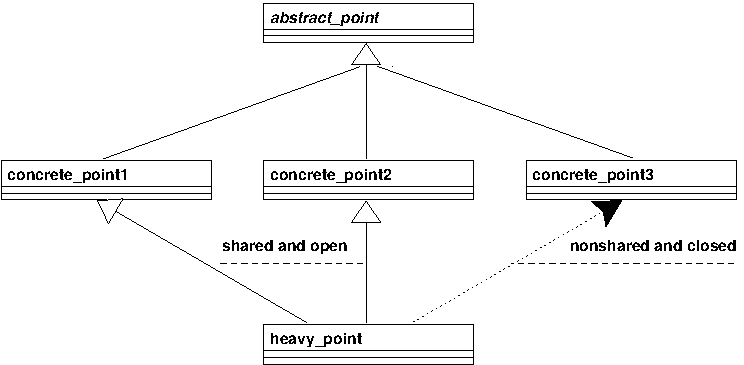
\includegraphics{heavy.pdf}}
\end{center}
\vspace{-33\in}
\caption{Diamond inheritance and beyond}
\label{F:heavy}
\end{figure*}



%%%%%%%%%%%%%%%%%%%%%%%%%%%%%%%%%%%%%%%%%%%%%%%%%%%%%%%%%%%%%%%%%%%%%%%%%%%%%
%%%%%%%%%%%%%%%%%%%%%%%%%%%%%%%%%%%%%%%%%%%%%%%%%%%%%%%%%%%%%%%%%%%%%%%%%%%%%
%%%%%%%%%%%%%%%%%%%%%%%%%%%%%%%%%%%%%%%%%%%%%%%%%%%%%%%%%%%%%%%%%%%%%%%%%%%%%



\subsection{Sophisticated inheritance boils down to record calculus}

In several OO languages, multiple inheritance is allowed. For
instance, in OCaml, the rules are as follows. Only the last definition
of a method is kept: the redefinition in a subclass of a method that
was visible in the parent class overrides the definition in the parent
class. Previous definitions of a method can be reused by binding the
related ancestor using a special \ldots @as@ \ldots notation.  The
bound name is said to be a pseudo value identifier that can only be
used to invoke an ancestor method. Other rules and notations exist for
Eiffel, C++, and so on.

In Haskell, we can handle more than plain multiple inheritance.
We are going to work through a scenario, where a class @heavy_point@
is constructed by inheritance from three different concrete subclasses
of @abstract_point@. The first two
concrete points will be shared in the resulting heavy point, because
we leave open the recursive knot. The third concrete point
does not participate in the open recursion; so it is not shared. See
Fig.~\ref{F:heavy} for an overview.

The object template for heavy points starts as follows:

\begin{code}
 heavy_point x_init color self =
  do
     super1 <- concrete_point1 x_init self
     super2 <- concrete_point2 x_init self
     super3 <- mfix (concrete_point3 x_init)
     ... -- to be continued
\end{code}

\noindent
That is, we bind all ancestor objects for subsequent reference. We
pass @self@ to the first two points, which participate in open
recursion, but we fix the third point in place. A heavy point carries
@print@ and @move@ methods that delegate corresponding messages to all
three points:

\begin{code}
     ... -- continued from above
     let myprint = do
                      putStr "super1: "; (super1 # print)
                      putStr "super2: "; (super2 # print)
                      putStr "super3: "; (super3 # print)
     let mymove  = ( \d -> do
                              super1 # move $ d
                              super2 # move $ d
                              super3 # move $ d )
     return 
       $    print  .=. myprint
      .*.   move   .=. mymove
      .*.   emptyRecord
     ... -- to be continued
\end{code}

\noindent
The three points, with all their many fields and methods, contribute
to the heavy point by means of left-biased union on records, which is
denoted by ``@.<++.@'' below:

\begin{code}
     ... -- continued from above
      .<++. super1
      .<++. super2
      .<++. super3
\end{code}

\noindent
(The routine definition of ``@.<++.@'' is given in App.~\ref{A:hLeftUnion}.)

\myskip

\noindent
It's time for a demo:

\begin{code}
 myDiamondOOP =
  do 
     p <- mfix (heavy_point 42 "blue")
     p # print -- All points still agree!
     p # move $ 2
     p # print -- The third point lacks behind!
\end{code}

\begin{code}
 ghci> myDiamondOOP
 super1: 42
 super2: 42
 super3: 42
 super1: 46
 super2: 46
 super3: 44
\end{code}



%%%%%%%%%%%%%%%%%%%%%%%%%%%%%%%%%%%%%%%%%%%%%%%%%%%%%%%%%%%%%%%%%%%%%%%%%%%%%
%%%%%%%%%%%%%%%%%%%%%%%%%%%%%%%%%%%%%%%%%%%%%%%%%%%%%%%%%%%%%%%%%%%%%%%%%%%%%
%%%%%%%%%%%%%%%%%%%%%%%%%%%%%%%%%%%%%%%%%%%%%%%%%%%%%%%%%%%%%%%%%%%%%%%%%%%%%



\subsection{No need for equi-recursive types}

We saw that our class constructor takes @self@ as an argument, and
returns the record, essentially @self'@, as the result. Our encoding
(for non-abstract classes) requires that @self@ and @self'@ have the
same slots -- but they do not have to be of the same type. This is how
we avoid recursive types. Later on, when we instantiate the class into
an object, we will apply @mfix@ operator -- that is, we will use value
recursion rather than the type recursion. Of course our technique
works if no method type involves the type of the self argument
(\emph{not} counting the implicit self). This is indeed the case in
most OO languages, where we must declare the type of the argument and
the result of a method, and that type must be a concrete type rather
than just `self'.  Functional objects obviously break this rule. We
have found a way to deal with functional objects while avoiding
recursive and existential types, but this topic is outside of the
scope of the present paper.



%%%%%%%%%%%%%%%%%%%%%%%%%%%%%%%%%%%%%%%%%%%%%%%%%%%%%%%%%%%%%%%%%%%%%%%%%%%%%
%%%%%%%%%%%%%%%%%%%%%%%%%%%%%%%%%%%%%%%%%%%%%%%%%%%%%%%%%%%%%%%%%%%%%%%%%%%%%
%%%%%%%%%%%%%%%%%%%%%%%%%%%%%%%%%%%%%%%%%%%%%%%%%%%%%%%%%%%%%%%%%%%%%%%%%%%%%
